%ltex: language=de-DE
\chapter{Vorbereitung}
	Um der zweigeteilten Natur des Praktikumsversuchs Sorge zu tragen wird die Diskussion der Vorbereitung in separaten Unterkapiteln
	erfolgen.
	\section{Kalorimetrischer Aufschluss}\label{sec:vorbereitung kalorimetrischer aufschluss}
		Versuch 11 beschäftigt sich mit der Theorie sowie der praktischen Durchführung eines kalorimetrischen Aufschlusses
		eines Paraffinöls, welches mit Chlorkohlenwasserstoff verunreinigt ist.\par
		Die durch vollständige Verbrennung frei gesetzte thermische Energie verteilt sich auf die direkt nutzbare und die durch
		etwa Verdampfung abtransportierte und für gewöhnlich verlorene Wärmemenge. Unter Einbezug auch der in der Dampfphase liegenden
		thermischen Energie wird in diesem Zusammenhang vom \textit{Brennwert} eines Stoffes gesprochen.
		Im vorliegenden Versuch soll unter Zuhilfenahme des Kalorimeters C 6000 der Firma \textsc{IKA} der Brennwert einer Paraffinprobe
		bestimmt werden.
		\begin{figure}[h]
			\centering
			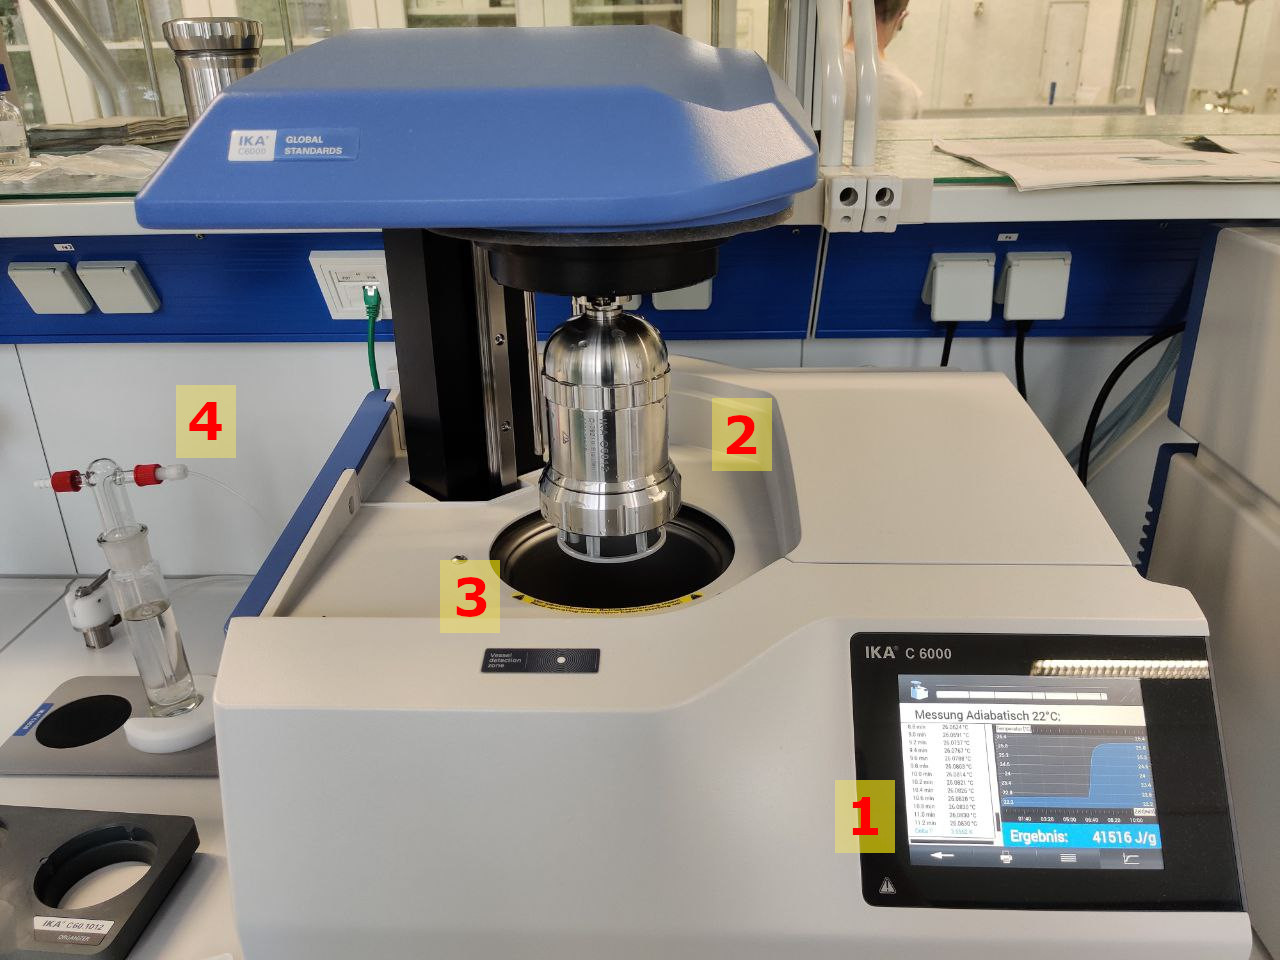
\includegraphics[width=.7\textwidth]{assets/photos/kaloriemeter_aufbau_edit.jpg}
			\caption[Im Versuch verwendetes Kalorimeter]{Im Versuch verwendetes Kalorimeter C 6000 der Firma \textsc{IKA}. Zu sehen 1: Bedienfeld, 2: Druckbehälter, 3: Innenkessel, 4: Entlüftungsstation.}
			\label{fig:kalorimeter aufbau}
		\end{figure}
		Das Funktionsprinzip besteht hierbei aus einer sehr genauen Messung der Temperaturerhöhung eines die Verbrennungskammer umfließenden
		Wassers. Da es hierbei unweigerlich auch Wärmemengenverlusten an den Gefäßwenden, Leitungen und dergleichen kommt, muss,
		um entsprechende Kompensationen durchführen zu können, im Vorfeld jeder Messung eine Kalibrierung durchgeführt werden.
		Die Kalibrierung bestimmt hier die Wärmekapazität der Messeinrichtung selbst und folgt der kalorischen Grundgleichung \cref{eq:kalorische grundgleichung} \cite{Einstieg.in.die.Physikalische.Chemie.fuer.Nebenfaechler.Bechmann.2016}.
		\begin{equation}
			Q = \Delta T \cdot k = \Delta T \cdot \sum_i c_i \cdot m_i
			\label{eq:kalorische grundgleichung}
		\end{equation}

		\(k = \sum_i c_i \cdot m_i\) bezeichnet hier einen systemspezifischen Proportionalitätsfaktor, der die kumulierte Fähigkeit der einzelnen Systemkomponenenten Wärme aufzunehmen
		widerspiegelt und muss durch Kalibrierung ermittelt werden. \(Q\) ist hier die zugeführte Wärmemenge und \(\Delta T\) die zu messende Temperaturänderung.\par\medskip
		\begin{figure}[h]
			\centering
			\includesvg[width=.6\textwidth]{assets/svg/paraffin_rein_struktur}
			\caption[Exemplarische Strukturformel reinen Paraffins]{Exemplarische Strukturformel reinen Paraffins.}
			\label{fig:paraffin rein}
		\end{figure}
		Sowohl die eigentliche Messung als auch die Kalibrierung finden unter Zufuhr reinen Sauerstoffs statt. Hierbei wird, wie eingangs bereits erwähnt, das Präparat
		vollständig verbrannt während die Temperaturänderung des umliegenden Wassers konstant gemessen wird.
		\Cref{fig:paraffin rein} und \ref{fig:paraffin ckw} zeigen exemplarische Strukturformeln jeweils eines reinen und eines mit Chlor modifizierten
		Paraffins.
		\begin{figure}[h]
			\centering
			\includesvg[width=.6\textwidth]{assets/svg/paraffin_ckw_struktur}
			\caption[Exemplarische Strukturformel eines mit Chlor verunreinigten Paraffins]{Exemplarische Strukturformel eines mit Chlor verunreinigten Paraffins.}
			\label{fig:paraffin ckw}
		\end{figure}\\
		Das in der kalorimetrischen Bestimmung verwendete Präparat ist ein Paraffin zweiten Typs. So wird beim Versuch über die Bestimmung des Brennwertes des
		Präparates hinaus auch der angelagerte Chlorgehalt bestimmt. Dies geschieht in einer nachgelagerten konduktometrischen Fällungstitration, die in \cref{sec:titration}
		näher erläutert werden soll.\par\medskip
		Um den beim Aufschluss zu erwartenden Chlorwasserstoff aufzufangen wird in Vorbereitung \SI{100}{mL} 0,1 molarer Natronlauge hergestellt.
		\begin{equation}
			\frac{c_{soll}(NaOH)}{V_{soll}} = \frac{c_1(NaOH)}{V} \qquad \Leftrightarrow \qquad V = c_1(NaOH) \cdot \frac{V_{soll}}{c_{soll}(NaOH)}
			\label{eq:verduennung}
		\end{equation}\\
		Im Versuch steht 1 molare Natronlauge zur Verfügung aus der die gewünschte Konzentration \(c_{soll}(NaOH)\) durch Verdünnung hergestellt werden muss. \Cref{eq:verduennung}
		folgend errechnet sich die zu entnehmende Menge zu \(V = \SI{10}{mL}\). Mit einer Vollpipette vorsichtig entnommen und in einen Messkolben überführt wird die Differenz
		zum Sollvolumen mit \SI{90}{mL} VE-Wasser aufgefüllt.\par\medskip
		%
		Die oben beschriebene Kalibrierung wird im Versuch durch Verbrennung von \SI{0,5}{g} Benzoesäure durchgeführt wobei die Kalibrierparameter

		\begin{addmargin}[8mm]{0pt}
			\texttt{Bezugsbrennwert}\\
			\texttt{Einwaage} und\\
			\texttt{QFremd1/2}
		\end{addmargin}
		bekannt sein müssen. \texttt{Bezugsbrennwert} ergibt sich aus dem spezifischen Brennwert der Benzoesäure mit \(H_0 = \SI{26,455}{\kilo\joule\per\kelvin}\) \cite{Versuchsanleitung.phys.chemie}.
		Die in Tablettenform vorgelegten Benzoesäure wird auf der Laborwaage im Tiegel eingewogen und ergibt so den Parameter \texttt{Einwaage} mit \(m_{Benz} = \SI{(506,8 \pm 1)}{mg}\).
		Ein sich ebenfalls im Tiegel befindlicher Baumwollfaden wird elektrisch entzündet und startet so die Verbrennung. Hierdurch werden allerdings zwei weitere Wärmeenergien eingebracht
		die durch Angabe des letzten Parameters \texttt{QFremd1/2} intern kompensiert werden. Hier wird \SI{120}{J} (Summe aus der Verbrennungsenergie des Baumwollfadens mit \(Q_{faden} = \SI{50}{J}\) und der
		des Zündfunkens mit \(Q_{funke} = \SI{70}{J})\) hinterlegt. Letztlich kann für die Kalibrierung ausgehend von \cref{eq:kalorische grundgleichung} geschrieben werden:
		\begin{equation}
			Q = H_0 \cdot m_{Benz} + Q_{faden} + Q_{funke} = \Delta T \cdot k
			\label{eq:grundgleichung fuer kalib umgeschrieben}
		\end{equation}

		mit \(k\) als der einzigen Unbekannten.\par
		Die im Zuge der Vorbereitung gemessene Kalorimeterkonstante \(k\) ergab sich zu
		\begin{equation}
			k = \SI{8025}{\joule\per\kelvin}
			\label{eq:kalorimeterkonstante}
		\end{equation}

		womit bei nachfolgenden Messungen der spezifische Brennwert \(H_0\) der unbekannten Probe ermittelt werden kann.
	\section{Konduktometrische Titration}\label{sec:titration}
		Liegt in einer Lösung nur eine Ionenart vor, so kann durch Neutralisation mit begleitender Überwachung der Leitfähigkeit der Lösung
		auf die anfängliche Ionenkonzentration geschlossen werden.

		Die Leitfähigkeit einer Lösung hängt in erster Linie von der Ionenbeweglichkeit (die wiederum in gewissem Maße auch von der Temperatur abhängt) und
		-konzentration ab. Die Leitfähigkeit hat dort ein Minimum, wo bei der Neutralisation ein Äquivalenzpunkt erreicht wird.
		Im vorliegenden Versuch wird nach dieser Methode der Chloridgehalt des Residuums aus Versuch 11 mittels Neutralisation mit einer Silbernitratlösung bestimmt.
		Da hierzu die Ionenkonzentration des Titranten möglichst genau bekannt sein muss, wird vorbereitend eine Lösung bekannten Chloridgehalts
		titriert. \nocite{Analytische.Chemie.I.Ritgen.2019}
		\begin{reaction}
			Na_{(aq)}^{+}Cl_{(aq)}^{-} + Ag_{(aq)}^{+}NO_{3(aq)}^{-} -> AgCl v + Na_{(aq)}^{+} + NO_{3(aq)}^{-}
			\label{re:NaCl und AgNO3}
		\end{reaction}
		\subsection*{Lösung bekannten Chloridgehaltes}\label{sec:bekannter chloridgehalt}
			Zur Herstellung einer Lösung bekannten Chloridgehalts wird Natriumchlorid (Kochsalz) auf der Laborwaage möglichst genau eingewogen
			und in einem Messkolben durch Auffüllen mit VE-Wasser gelöst. Ziel ist eine Chloridkonzentration von \(c(Cl^{-}) \approx \SI{0,1}{\mole\per\litre}\).
			\begin{equation}
				m = \left[M(Cl^{-}) + M(Na^{+})\right] \cdot c(Cl^{-}) \cdot V
				\label{eq:masse NaCl}
			\end{equation}

			Mit den molaren Massen von \(M(Cl^{-}) \approx \SI{35,450}{\gram\per\mole}\) und \(M(Na^{+}) \approx \SI{22,98977}{\gram\per\mole}\) sowie
			dem herzustellenden Volumen von \(V = \SI{50}{\milli\litre}\) ergibt sich mit \cref{eq:masse NaCl} eine einzuwiegende Masse des Salzes
			von gemäß \SI{292,2}{mg}. Mit einer tatsächlich eingewogenen Masse von\\
			\(\SI{(298,8 \pm 0,1)}{\milli\gram}\) führt dies wiederum gemäß \cref{eq:konzentration Cl}
			\begin{equation}
				c(Cl^-) = \frac{M(Cl^-)}{M(Cl^-) + M(Na^+)} \cdot \frac{m}{M(Cl^-) \cdot V}
				\label{eq:konzentration Cl}
			\end{equation}
			zu einer Konzentration von \(c(Cl^{-}) \approx \SI{0,1023}{\mole\per\litre}\).\par
			Von der hergestellten Lösung werden \SI{25}{\milli\litre} entnommen und innerhalb eines Becherglases mit \SI{200}{\milli\litre}
			VE-Wasser verdünnt.
		\subsection{Titerbestimmung}\label{sec:titerbestimmung}
			Das Becherglas aus \cref{sec:bekannter chloridgehalt} wird mit einem Rührstäbchen versehen auf einen Magnetrührer gestellt und
			das in einem Stab kombinierte Elektrodenpaar des Konduktometers in einem über dem Becherglas befindlichen Stativ so arretiert, dass
			die Kontaktflächen der Elektroden möglichst tief in die Lösung eintauchen\footnote{Hierbei ist darauf zu achten, dass der Elektrodenstab möglichst frei von Kontamination ist.}.

			Nach Einschalten des Magnetrührers wird \SI{2}{\milli\litre}-Schritten Silbernitratlösung zu titriert und bei jedem Titrationsschritt die
			momentane Leitfähigkeit der Lösung am Konduktometer abgelesen und aufgezeichnet. Nahe des Äquivalenzpunktes werden die Titrationsschritte auf
			etwa \SI{0,5}{\milli\litre} reduziert um das Minimum der Leitfähigkeit möglichst genau zu lokalisieren. Ist der Äquivalenzpunkt erreicht wird die Schrittweite
			der Titration wieder erhöht und so lange Silbernitratlösung zugegeben, bis etwa \SI{20}{\milli\litre} nach dem Äquivalenzpunkt verbraucht sind.